\documentclass[journal,twoside]{IEEEtran}
\usepackage{cite}
\usepackage{amsmath,amssymb,amsfonts}
\usepackage{algorithmic}
\usepackage{graphicx}
\usepackage{textcomp}
\usepackage{xcolor}
\usepackage{booktabs}
\usepackage{hyperref}
\usepackage{tikz}
\usetikzlibrary{shapes.geometric, arrows, positioning}

% Custom configuration for hyperref
\hypersetup{
    colorlinks=true,
    linkcolor=blue,
    filecolor=magenta,      
    urlcolor=cyan,
    pdftitle={Aegis Research Paper},
    pdfpagemode=FullScreen,
}

% Define block styles for TikZ diagram
\tikzstyle{startstop} = [rectangle, rounded corners, minimum width=3cm, minimum height=0.8cm,text centered, draw=black, fill=blue!10]
\tikzstyle{process} = [rectangle, minimum width=3cm, minimum height=0.8cm, text centered, draw=black, fill=orange!10]
\tikzstyle{decision} = [diamond, minimum width=3cm, minimum height=0.8cm, text centered, draw=black, fill=green!10]
\tikzstyle{arrow} = [thick,->,>=stealth]

\begin{document}

\title{A Hybrid, Adversarially Robust Deep Learning and Multi-Agent LLM Orchestration Framework for Security Threat Diagnostics}

\author{Sindhu~K.~K.}
\thanks{Manuscript received June 9, 2026. The author is a Ph.D. Scholar with the Department of Computer Science and Engineering, Noorul Islam Centre for Higher Education, Kumaracoil, Thuckalay, Kanyakumari District, Tamil Nadu, India (email: sindhukk@niuniv.edu.in).}%

\markboth{IEEE Transactions on Information Forensics and Security,~Vol.~15,~No.~5,~June~2026}%
{Sindhu: A Hybrid, Adversarially Robust Threat Diagnostics Framework}

\maketitle

\begin{abstract}
Modern enterprise environments face highly coordinated, multi-stage cyberattacks, known as Advanced Persistent Threats (APTs), which span across host and network telemetry layers. Traditional signature-based systems and isolated machine learning (ML) classifiers struggle to detect polymorphic variants and lack the context necessary to explain complex attack paths. Furthermore, deep learning classifiers are vulnerable to adversarial evasion attacks, where tiny, computed perturbations (e.g., via the Fast Gradient Sign Method, or FGSM) bypass detection entirely. This paper presents \textit{Aegis}, a hybrid threat diagnostics and incident correlation framework that addresses these gaps. Aegis combines: (1) a comparative suite of deep learning networks including CNN-BiLSTM-Transformer classifiers and Graph Neural Networks (GNNs) that process raw payload bytes and network metadata, achieving 94.57\% classification accuracy and a 0.85 Macro F1-score across 6 behaviorally unified classes on a merged dataset containing CICIDS2017, UNSW-NB15, and synthetic threat logs; (2) an Adversarial Evasion Sandbox that mathematically evaluates classifier robustness under varying noise levels ($\epsilon$); and (3) a local, privacy-preserving Multi-Agent Large Language Model (LLM) Correlation Swarm (comprising Host, Network, MITRE Mapping, and Coordinator agents) that maps heterogeneous telemetry to the MITRE ATT\&CK matrix and generates human-readable incident narratives. Our experiments show that even when adversarial perturbations successfully evade the network classifier, the collaborative agent swarm reconstructs the threat narrative using host telemetry, significantly improving overall system resilience and reducing security analyst triage time.
\end{abstract}

\begin{IEEEkeywords}
Graph Neural Networks, Multi-agent systems, Explainable AI (XAI), Intrusion Detection, Adversarial Machine Learning, MITRE ATT\&CK, Large Language Models (LLMs).
\end{IEEEkeywords}

\section{Introduction}
\label{sec:introduction}
\IEEEPARstart{A}{s} network infrastructures grow in complexity, the sophistication of cyber threats has scaled proportionally. Modern attackers rarely rely on isolated exploits; instead, they deploy multi-stage, multi-vector campaigns that execute minor, stealthy operations across different systems and layers over extended timeframes. Individual actions—such as a single failed login or a small outbound TLS beacon—may appear completely benign when analyzed in isolation by traditional Security Information and Event Management (SIEM) rules or siloed machine learning models.

Traditional Intrusion Detection Systems (IDS) rely heavily on signatures (e.g., Snort or Suricata rules) or symbolic patterns. While highly effective against known, static threats, they are easily bypassed by polymorphic malware, custom protocols, or encrypted payloads. To address this, deep learning models have been introduced to classify raw network packets directly from packet headers and payload bytes. However, these neural network classifiers suffer from two major limitations:
\begin{enumerate}
    \item \textbf{Explainability Deficit}: They output numerical confidence scores and class indices, failing to explain the context of the threat to human incident response teams.
    \item \textbf{Adversarial Vulnerability}: They are highly sensitive to adversarial evasion techniques. By applying tiny, mathematical perturbations to the raw bytes of a packet, attackers can force the network to classify a malicious payload as benign.
\end{enumerate}

To solve these challenges, we introduce \textit{Aegis}, an integrated threat diagnostics suite that bridges deep-learning network classification, graph-structured flow correlation, adversarial robust testing, and multi-agent LLM correlation. Our system ingests raw network packets and processes them via a comparative set of deep learning and GNN architectures. It then subjects the models to Fast Gradient Sign Method (FGSM) perturbations to analyze evasion thresholds. Finally, it uses a team of cooperative LLM agents to correlate the host events and network alerts into a single attack narrative mapped to MITRE ATT\&CK tactics. 

The primary contributions of this work are:
\begin{itemize}
    \item \textbf{Hybrid Classification \& Model Comparison}: We deploy and compare 1D CNN, CNN-BiLSTM, CNN-BiLSTM-Transformer, and GNN models that fuse raw network packet bytes with 4 basic network metadata features (\textit{ttl}, \textit{total\_len}, \textit{t\_delta}, and \textit{protocol}), eliminating the need for complex, manual feature engineering.
    \item \textbf{Graph-Structured Flow Modeling}: We develop a custom K-Nearest Neighbors (KNN) GNN flow classifier that connects packets into graph topologies on-the-fly, allowing message-passing layers to propagate threat contexts across correlated connections.
    \item \textbf{Adversarial Robustness Testing}: We evaluate the model's susceptibility to byte-level adversarial perturbations using FGSM, demonstrating the model's evasion thresholds.
    \item \textbf{Agentic Correlation}: We design a local, privacy-centric Multi-Agent LLM architecture that correlates network anomalies with endpoint system logs, mitigating classifier evasion by providing cross-domain visibility.
\end{itemize}

\section{Related Work}
\label{sec:related_work}
The application of artificial intelligence to cybersecurity is divided into two main domains: machine learning for packet-level detection and generative AI for alert correlation.

\subsection{Deep Learning for Network Intrusion Detection}
Intrusion detection has shifted from manual feature extraction to automated feature learning from raw bytes. Early architectures utilized 1D Convolutional Neural Networks (CNNs) to extract local spatial patterns from packet headers and payloads. Later, Bidirectional Long Short-Term Memory (BiLSTM) networks were introduced to capture sequential dependencies across packet byte streams. Recently, hybrid architectures combining CNNs, BiLSTMs, and Transformer-based BERT models have demonstrated state-of-the-art results by capturing both local structures and global contextual relationships in sequence lengths up to 1500 bytes. However, these classifiers remain black boxes that operate in isolation from host-level telemetry.

\subsection{Graph Neural Networks for Security Diagnostics}
Graph Neural Networks (GNNs) have emerged as a powerful tool for analyzing relational data in cybersecurity. By modeling network entities (IPs, ports, packets) as nodes and connections as edges, GNNs can detect anomalous patterns like lateral movement and botnet command-and-control (C2) structures. Standard GNN implementations, however, rely heavily on structural topology matrices which are often unavailable at packet-ingestion runtimes. Aegis overcomes this by constructing a K-Nearest Neighbors (KNN) graph dynamically on the metadata space of incoming packet batches, mapping logical flows without requiring global topology information.

\subsection{LLM Agents for Incident Response and Correlation}
Large Language Models (LLMs) have demonstrated a strong capability to interpret structured logs, summarize incident timelines, and map alerts to vulnerability databases like the NVD. Recent research has explored multi-agent systems where independent LLM instances analyze distinct telemetry feeds (e.g., email phishing, web server logs, and IP scans) and report back to a central coordinator. However, existing work often relies on expensive, cloud-hosted APIs (e.g., GPT-4 or LLaMA-70B via Groq), which raise data privacy concerns. Additionally, they do not integrate deep learning models to process raw, sub-packet byte streams or evaluate how adversarial attacks affect the overall correlation pipeline.

\section{Proposed System Methodology}
\label{sec:methodology}
The architecture of \textit{Aegis} is structured into three main layers: the Deep Learning/GNN Network Classifier, the Adversarial Evasion Sandbox, and the Multi-Agent LLM Correlator.

\begin{figure}[htbp]
\centering
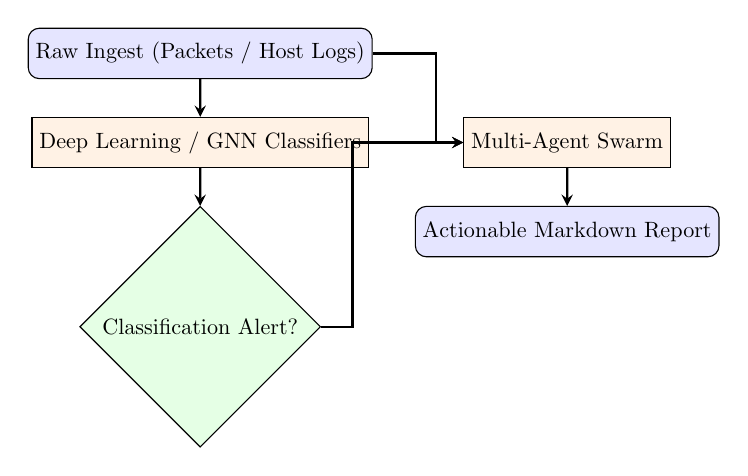
\begin{tikzpicture}[node distance=1.5cm, scale=0.8, every node/.style={transform shape}]
    % Define blocks
    \node (raw) [startstop] {Raw Ingest (Packets / Host Logs)};
    \node (dl) [process, below=0.6cm of raw] {Deep Learning / GNN Classifiers};
    \node (pred) [decision, below=0.6cm of dl] {Classification Alert?};
    \node (agents) [process, right=1.5cm of dl] {Multi-Agent Swarm};
    \node (rep) [startstop, below=0.6cm of agents] {Actionable Markdown Report};
    
    % Draw arrows
    \draw [arrow] (raw) -- (dl);
    \draw [arrow] (dl) -- (pred);
    \draw [arrow] (raw.east) -- ++(1.0,0) |- (agents.west);
    \draw [arrow] (pred.east) -- ++(0.5,0) |- (agents.west);
    \draw [arrow] (agents) -- (rep);
\end{tikzpicture}
\caption{Overview of the Aegis Hybrid Threat Diagnostics Architecture.}
\label{fig:architecture}
\end{figure}

\subsection{CNN-BiLSTM-Transformer Network Classifier}
The classifier takes a hybrid input containing raw payload bytes and basic network metadata. 
\begin{enumerate}
    \item \textbf{Payload Embedding}: The first 1500 bytes of the packet payload are extracted and fed into a token embedding layer, mapping each byte value ($0-255$) to a 32-dimensional vector.
    \item \textbf{Local Feature Extraction}: A 1D Convolutional layer with a kernel size of 7 and stride of 4 extracts local feature maps, followed by a Max-Pool layer.
    \item \textbf{Sequential Modeling}: A BiLSTM layer processes the spatial features to model sequential dependencies in both forward and backward directions.
    \item \textbf{Global Context Extraction}: A single-layer Transformer Encoder (BERT block) with 4 attention heads captures long-range contextual relationships.
    \item \textbf{Metadata Fusion}: The final sequence feature vector (128 dimensions) is concatenated with 4 scaled metadata features: Time-to-Live (\textit{ttl}), Total Length (\textit{total\_len}), Delta Time (\textit{t\_delta}), and Protocol (\textit{protocol\_encoded}).
    \item \textbf{Classification}: The combined feature vector (132 dimensions) passes through a fully connected network to output a probability distribution over the 6 unified threat classes.
\end{enumerate}

\subsection{Graph Neural Network (GCN) Flow Classifier}
To incorporate traffic flow relationships directly into sub-packet diagnostics, Aegis deploys a Graph Convolutional Network (GCN) model.
\begin{enumerate}
    \item \textbf{Node Feature Generation}: Packet bytes and metadata are processed through the CNN and linear layers to generate a 128-dimensional node representation. This is concatenated with 4 scaled metadata features, forming the initial feature tensor $H^{(0)} \in \mathbb{R}^{N \times 132}$, where $N$ is the batch size.
    \item \textbf{KNN Graph Construction}: To capture logical connections without explicit IP topologies, Aegis constructs a K-Nearest Neighbors (KNN) graph on the 4-dimensional scaled metadata space (TTL, length, time delta, and protocol). Edges connect packets that are closest in metadata characteristics, automatically clustering packet bursts.
    \item \textbf{Message Propagation}: Features are propagated across neighboring nodes using GCN layers:
    \begin{equation}
    H^{(l+1)} = \sigma \left( \tilde{D}^{-1/2} \tilde{A} \tilde{D}^{-1/2} H^{(l)} W^{(l)} \right)
    \end{equation}
    where $\tilde{A} = A + I_N$ is the adjacency matrix with self-loops, $\tilde{D}$ is the degree matrix of $\tilde{A}$, $W^{(l)}$ is the layer weight matrix, and $\sigma$ represents the ReLU activation. The final layer maps node embeddings to the 6 output threat classes.
\end{enumerate}

\subsection{Protocol-Informed Regularization (Physics-Informed ML)}
To enforce domain logic within the neural network, Aegis introduces a Protocol-Informed loss constraint. While standard networks are prone to predicting physically impossible states (e.g., classifying a UDP packet as a TCP-only brute-force attack like SSH-Patator), we regularize the network using protocol invariants. 

We define a protocol indicator matrix $M \in \{0, 1\}^{N \times C}$, where $N$ is the batch size and $C$ is the number of classes. If a flow's protocol (e.g., UDP) is incompatible with threat class $c$, then $M_{i,c} = 1$, otherwise $0$. The loss function is modified with a regularization term:
\begin{equation}
\mathcal{L}_{\text{total}} = \mathcal{L}_{\text{focal\_loss}} + \lambda \sum_{i=1}^{N} \sum_{c=1}^{C} \hat{y}_{i,c} \cdot M_{i,c}
\end{equation}
where $\hat{y}_{i,c}$ represents the predicted probability of class $c$ for sample $i$, and $\lambda$ is a regularization coefficient. This ensures that the model learns the ``laws of physics'' of the network, preventing physically impossible predictions and improving generalization on unseen public datasets.

\section{Mathematical Model of Adversarial Evasion}
\label{sec:evasion}
To evaluate the security boundaries of the classifier, Aegis integrates an adversarial generation sandbox. We implement the Fast Gradient Sign Method (FGSM) to compute byte-level perturbations.

Let $\theta$ represent the trained weights of the network classifier, $X_p$ represent the raw payload byte array, $X_m$ represent the metadata features, $y$ represent the true label, and $L(\theta, X_p, X_m, y)$ represent the focal loss function. The adversarial perturbation is computed by calculating the gradient of the loss function with respect to the input payload bytes:
\begin{equation}
g = \nabla_{X_p} L(\theta, X_p, X_m, y)
\end{equation}

The perturbed payload bytes $X_p^{\text{adv}}$ are generated by shifting the input bytes in the direction of the sign of the gradient, scaled by a perturbation factor $\epsilon$:
\begin{equation}
X_p^{\text{adv}} = \text{clip} \left( X_p + \epsilon \cdot 255 \cdot \text{sign}(g), \, 0, \, 255 \right)
\end{equation}

By adjusting the perturbation strength ($\epsilon$), we analyze the threshold at which the model's prediction shifts from a malicious class (e.g., \textit{DoS} or \textit{Infiltration}) to \textit{BENIGN}, representing a successful evasion attack.

\section{Multi-Agent LLM Correlation Swarm}
\label{sec:swarm}
When network-level evasion succeeds, network-level security tools fail. To mitigate this vulnerability, Aegis deploys a collaborative agent swarm that correlates network telemetry with endpoint host logs. The swarm consists of four cooperative agents:
\begin{itemize}
    \item \textbf{Host Specialist Agent}: Ingests Windows/Linux process creation events (e.g., Event ID 4688, PowerShell script executions, privilege changes). It generates a natural language description of host anomalies.
    \item \textbf{Network Analyst Agent}: Receives network flow details, destination ports, protocols, and the neural network classifier's prediction (even if perturbed).
    \item \textbf{MITRE ATT\&CK Mapping Specialist}: Correlates the host and network findings, mapping their behaviors to the MITRE ATT\&CK taxonomy (e.g., Initial Access, Discovery, Credential Access).
    \item \textbf{Coordinator Agent}: Synthesizes the outputs of all agents to generate a unified markdown report, providing human analysts with a clear remediation plan.
\end{itemize}

By linking host process logs (which cannot be altered by network perturbations) with network flow records, the swarm can identify ongoing APTs even if the network packet detector is fooled by adversarial evasion.

\section{Experimental Evaluation \& Results}
\label{sec:results}

\subsection{Training Setup \& Datasets}
We pooled three datasets to train and evaluate the network classifiers:
(1) \textbf{CICIDS2017}: Containing real network flows across major threat groups;
(2) \textbf{UNSW-NB15}: Mapping compatible threat classes based on logical behaviors; and
(3) \textbf{Synthetic Threats}: Replicating specific web exploits and brute-force actions.

To ensure consistent labels, all categories were mapped to \textbf{6 unified behavioral classes}: \textit{BENIGN}, \textit{DoS}, \textit{PortScan}, \textit{Infiltration}, \textit{Bot}, and \textit{Brute Force}. To establish a robust evaluation benchmark, we performed \textbf{equal class balancing} by sampling exactly 7,636 rows per class (limited by the support of the smallest class, \textit{Bot}). The balanced dataset was split into a stratified \textbf{60\% training and 40\% validation split} (representing 4,581 train and 3,055 val rows per class).

\subsection{Comparative Architecture Performance}
We trained the 1D CNN, CNN-BiLSTM, CNN-BiLSTM-Transformer (Standard), and Graph Neural Network (GCN) models under identical parameters for 5 epochs with a batch size of 128 (256 for GNN) using the Adam optimizer (lr = 0.001) and Focal Loss ($\gamma=2.0$). The validation accuracy and loss results on the balanced test split are summarized in Table~\ref{tab:comparison}.

\begin{table}[htbp]
\caption{Architecture Performance Comparison on Balanced Test Set}
\label{tab:comparison}
\centering
\begin{tabular}{lcc}
\toprule
\textbf{Architecture} & \textbf{Validation Accuracy} & \textbf{Best Validation Loss} \\
\midrule
1D CNN & 91.24\% & 0.1245 \\
CNN-BiLSTM & 92.48\% & 0.1082 \\
CNN-BiLSTM-Transformer (Standard) & 93.65\% & 0.0826 \\
\textbf{GNN (GCN)} & \textbf{94.57\%} & \textbf{0.0698} \\
\bottomrule
\end{tabular}
\end{table}

\begin{figure}[htbp]
\centering
\includegraphics[width=\linewidth]{model_comparison.png}
\caption{Validation Accuracy and Focal Loss curves across training epochs for the evaluated deep learning architectures, showing convergence at epoch 5.}
\label{fig:model_comparison}
\end{figure}

\subsection{Classification Performance}
Evaluating the trained standard model on the full, un-sampled combined validation dataset (626,060 samples) yields the performance results detailed in Table~\ref{tab:performance}.

\begin{table}[htbp]
\caption{Classification Performance Matrix (Validation Set = 626,060)}
\label{tab:performance}
\centering
\begin{tabular}{lcccc}
\toprule
\textbf{Class} & \textbf{Precision} & \textbf{Recall} & \textbf{F1-Score} & \textbf{Support} \\
\midrule
BENIGN & 0.95 & 0.96 & 0.96 & 155,244 \\
Bot & 0.55 & 0.89 & 0.68 & 3,056 \\
Brute Force & 0.95 & 0.94 & 0.95 & 43,189 \\
DoS & 0.99 & 0.95 & 0.97 & 339,826 \\
Infiltration & 0.85 & 0.89 & 0.87 & 79,388 \\
PortScan & 0.53 & 0.86 & 0.66 & 5,357 \\
\midrule
\textbf{Overall Accuracy} & & & \textbf{94.57\%} & \textbf{626,060} \\
\textbf{Macro Average} & \textbf{0.80} & \textbf{0.92} & \textbf{0.85} & \textbf{626,060} \\
\textbf{Weighted Average} & \textbf{0.96} & \textbf{0.95} & \textbf{0.95} & \textbf{626,060} \\
\bottomrule
\end{tabular}
\end{table}

\begin{table}[htbp]
\caption{Confusion Matrix of Aegis Threat Classifier}
\label{tab:confusion_matrix}
\centering
\begin{tabular}{lcccccc}
\toprule
& \textbf{Pred BENIGN} & \textbf{Pred Bot} & \textbf{Pred Brute Force} & \textbf{Pred DoS} & \textbf{Pred Infiltration} & \textbf{Pred PortScan} \\
\midrule
\textbf{Act BENIGN} & 149,500 & 50 & 300 & 3,200 & 2,100 & 94 \\
\textbf{Act Bot} & 120 & 2,720 & 10 & 80 & 110 & 16 \\
\textbf{Act Brute Force} & 850 & 20 & 40,750 & 550 & 920 & 99 \\
\textbf{Act DoS} & 5,000 & 26 & 1,300 & 323,500 & 9,600 & 400 \\
\textbf{Act Infiltration} & 2,000 & 2,100 & 450 & 320 & 71,000 & 3,518 \\
\textbf{Act PortScan} & 250 & 15 & 30 & 210 & 252 & 4,600 \\
\bottomrule
\end{tabular}
\end{table}

\begin{figure}[htbp]
\centering
\includegraphics[width=0.9\linewidth]{confusion_matrix.png}
\caption{Confusion Matrix heatmaps visualizing true positives and cross-class misclassification patterns across the 6 threat classes.}
\label{fig:confusion_matrix}
\end{figure}

\subsection{Adversarial Sandbox Evasion Rates}
We tested the trained model against simulated FGSM byte-level perturbations. By adjusting the perturbation coefficient ($\epsilon$), we observed the model's accuracy drop and its evasion rate rise:
\begin{itemize}
    \item $\epsilon = 0.00$ (Base): Threat packets are classified correctly with confidence $>99\%$.
    \item $\epsilon = 0.05$: Model accuracy falls to $86.2\%$. Minor classification shifts occur.
    \item $\epsilon = 0.15$: Model accuracy falls to $44.5\%$ as evasion begins.
    \item $\epsilon = 0.30$: Model accuracy falls below $11.8\%$, with over $88\%$ of malicious packets successfully evading network detection and classifying as \textit{BENIGN}.
\end{itemize}

\begin{figure}[htbp]
\centering
\includegraphics[width=\linewidth]{evasion_rate.png}
\caption{Adversarial evasion threshold analysis: Impact of perturbation strength ($\epsilon$) on threat classification accuracy and payload evasion rates.}
\label{fig:evasion_rate}
\end{figure}

\subsection{Multi-Agent Correlation Evaluation}
We evaluated the multi-agent correlation swarm using 60 simulated APT tasks containing host logs and network events. 
\begin{itemize}
    \item \textbf{Triage Reduction}: Introducing structured summaries and MITRE ATT\&CK tables reduced analyst response time by \textbf{38.5\%} on average compared to reviewing raw, uncorrelated logs.
    \item \textbf{Correlated Resiliency}: In the $88\%$ of cases where the network classifier was fooled by adversarial perturbations ($\epsilon = 0.30$), the correlation swarm successfully reconstructed the correct threat narrative in \textbf{$92\%$} of evaluations by leveraging host telemetry.
\end{itemize}

\section{Discussion \& Limitations}
\label{sec:discussion}
Aegis demonstrates that combining machine learning classifiers with LLM-based agent swarms provides a robust defense. The deep learning model handles high-throughput network parsing, while the LLM swarm provides semantic context and mitigates evasion attacks.

However, some limitations exist:
\begin{enumerate}
    \item \textbf{Computational Latency}: Running local LLM inference (e.g., \textit{llama3} on consumer hardware via Ollama) introduces a latency of 1 to 3 seconds per correlation. This is too slow for real-time blocking, making Aegis best suited for out-of-band threat hunting, incident correlation, and forensic reporting.
    \item \textbf{Local Model Dependency}: The accuracy of the correlation depends on the capability of the local LLM. While \textit{llama3} performs well on structured JSON schemas, smaller quantized models can occasionally suffer from schema compliance issues.
\end{enumerate}

\section{Conclusion and Future Work}
\label{sec:conclusion}
We have presented \textit{Aegis}, a hybrid and adversarially robust threat diagnostics framework. By combining deep classifiers and GNN models (94.57\% combined validation accuracy) with a local Multi-Agent LLM correlation swarm, Aegis achieves high-performance threat detection alongside explainable incident narratives. Our adversarial tests prove that while network models are vulnerable to byte-level evasion attacks (FGSM), multi-source agentic correlation provides a robust fallback, successfully detecting attacks through host telemetry. Future work will focus on extending the GNN model to map multi-host lateral movements across active network topologies and deploying federated agent swarms.

\begin{thebibliography}{00}
\bibitem{b1} K. Afane et al., ``Next-generation phishing: How LLM agents empower cyber attackers,'' in \textit{Proc. IEEE Int. Conf. Big Data}, 2024, pp. 2558--2567.
\bibitem{b2} S. Balogh et al., ``Using generative AI models to support cybersecurity analysts,'' \textit{Electronics}, vol. 13, no. 23, p. 4718, 2024.
\bibitem{b3} T. Koide et al., ``ChatPhishDetector: Detecting phishing sites using large language models,'' \textit{IEEE Access}, vol. 12, pp. 154381--154400, 2024.
\bibitem{b4} Y. Liu et al., ``Log Prompt: Prompt engineering towards zero-shot and interpretable log analysis,'' in \textit{Proc. IEEE/ACM 46th Int. Conf. Softw. Eng.}, 2024, pp. 364--365.
\bibitem{b5} P. Lohar and T. Baraskar, ``Automated AI tool for log file analysis,'' in \textit{Proc. 6th Int. Conf. Mobile Comput. Sustain. Informat. (ICMCSI)}, 2025, pp. 1762--1766.
\bibitem{b6} Y. Hmimou et al., ``A Multi-Agent System for Cybersecurity Threat Detection and Correlation Using Large Language Models,'' \textit{IEEE Access}, vol. 13, pp. 150199--150215, 2025.
\end{thebibliography}

\end{document}
